\chapter{Marco Te\'{o}rico}
En esta secci\'{o}n se presenta el marco te\'{o}rico de la investigaci\'{o}n. En la primera parte se muestra el marco conceptual, en el cual se incluyen definiciones importantes sobre los c\'{i}tricos, su producci\'{o}n, sus especies y las respectivas enfermedades, adem\'{a}s de las normas que actualmente se est\'{a}n utilizando en la producci\'{o}n y mantenimiento de estas especies, las cuales nos ayudar\'{a}n a entender la importancia de este trabajo en la industria de los c\'{i}tricos. En la segunda parte se presenta lo concerniente a los temas o definiciones estad\'{i}sticas, como la teor\'{i}a de los diferentes tipos de muestreo que se podr\'{i}an aplicar en campo; el muestreo de aceptaci\'{o}n/rechazo y sus diferentes distribuciones y par\'{a}metros a tener en cuenta, y finalmente, algunas medidas de desempe\~{n}o que nos ayudar\'{a}n a elegir entre diferentes planes de muestreo propuestos.

\section{Marco Conceptual}
~\\\textbf{C\'{i}tricos}

Los c\'{i}tricos designan las especies de grandes arbustos o arbolillos perennes (entre 5 y 15 m) cuyos frutos o frutas, poseen un alto contenido en vitamina C y \'{a}cido c\'{i}trico. Los c\'{i}tricos pertenecen a la familia \textit{Rutaceae} y se encuentran agrupados en la subfamilia \textit{Aurantioideae}. Los g\'{e}neros m\'{a}s importantes son: \textit{Citrus}, \textit{Poncirus} y \textit{Fortunela}. Las especies del g\'{e}nero \textit{Citrus} son las m\'{a}s importantes desde el punto de vista agron\'{o}mico y representan casi la totalidad de los c\'{i}tricos cultivados.

~\\\textbf{Clasificac\'{o}n de los c\'{i}tricos}

El g\'{e}nero \textit{Citrus} ha sido clasificado por los tax\'{o}nomos de diferentes maneras. Normalmente se utiliza la clasificaci\'{o}n de \textit{Swingle}. Las especies m\'{a}s conocidas y cultivadas son las siguientes: 
\begin{itemize}
\item \textit{Citrus aurantifolia} (Christon.) Swing. Conocido en el comercio internacional como lima mejicana, y en Colombia, como lim\'{o}n pajarito o de Castilla, aunque bot\'{a}nicamente es una lima \'{a}cida.
\item \textit{Citrus latifolia} Tanaka. Lima Tahit\'{i}
\item \textit{Citrus aurantium} L. Naranjo amargo
\item \textit{Citrus grandis} (L.) Osb. Pummelo
\item \textit{Citrus limon} (L.) Burm. Lim\'{o}n verdadero
\item \textit{Citrus paradisi} Macf. Toronja o pomelo
\item \textit{Citrus reticulata} Blanco. Mandarina
\item \textit{Citrus sinensis} (L.) Osb. Naranjo dulce
\end{itemize}

~\\\textbf{Resoluci\'{o}n ICA 4215, 2014}

Es la norma ``por medio de la cual se establecen los requisitos para el registro de los viveros y/o huertos b\'{a}sicos productores y/o comercializadores de semilla sexual y/o asexual (material vegetal de propagaci\'{o}n) de c\'{i}tricos y se dictan otras disposiciones''. En esta norma se dan un conjunto de definiciones agron\'{o}micas y se establecen los requisitos formales y de infraestructura que deben tener los viveros para registrarse ante el ICA. Se dictan distintas disposiciones para evitar una mala calidad o infecciones en las plantas, por ejemplo, las plantas deben estar en casa de malla a una altura de 15 cms del suelo para evitar la entrada de \'{a}fidos o pulgones que esparcen las diversas enfermedades.

De aqu\'{i} se desprenden diferentes conceptos importantes para el desarrollo de este trabajo:
\begin{itemize}
\item Vivero: \'{A}rea de terreno delimitada para propagar semillas de c\'{i}tricos [Resoluci\'{o}n ICA 4215, 2014]
\end{itemize}

Seg\'{u}n la FAO, 1990:
\begin{itemize}
\item Lote: Conjunto de unidades de un solo producto b\'{a}sico, identificable por su composici\'{o}n homog\'{e}nea, origen, etc., que forma parte de un env\'{i}o.
\item Plaga: Cualquier especie, raza o biotipo vegetal o animal o agente pat\'{o}geno da\~{n}ino para las plantas o productos vegetales.
\item Prueba: Examen oficial, no visual, para determinar la presencia de plagas o para identificar tales plagas. 
\end{itemize}

~\\\textbf{Enfermedades en los c\'{i}tricos}

En Colombia los cultivos de c\'{i}tricos pueden ser atacados por varias especies de insectos y \'{a}caros da\~{n}inos, que afectan el desarrollo de los \'{a}rboles, limitan su producci\'{o}n y disminuyen la calidad de la fruta. Los costos de las pr\'{a}cticas utilizadas para controlar y evitar los da\~{n}os causados por plagas, influyen en la rentabilidad econ\'{o}mica de las explotaciones citr\'{i}colas comerciales. Algunas de las enfermedades m\'{a}s frecuentes y de mayor cuidado son: 
\begin{itemize}
\item Virus de la tristeza: El virus de la tristeza de los c\'{i}tricos (Citrus tristeza virus, CTV) causa una de las enfermedades m\'{a}s
da\~{n}inas de este cultivo. Se refiere al decaimiento observado en muchas especies de c\'{i}tricos injertados sobre patrones de Citrus aurantium (naranjo amargo) o de Citrus limon (limonero); algunas cepas del CTV inducen otros s\'{i}ndromes, como acanaladuras o picado del tallo, enanismo, menor productividad y baja calidad del fruto en muchos cultivares comerciales,incluso en ejemplares injertados sobre patrones tolerantes a la tristeza.\cite{CTV}
\item Huanglongbing(HLB):Es una de las enfermedades m\'{a}s peligrosas y temidas por las p\'{e}rdidas productivas y econ\'{o}micas que ocasiona. Las plantas j\'{o}venes afectadas no entran nunca en producci\'{o}n y las plantas adultas dejar\'{a}n de producir pocos a\~{n}os despu\'{e}s de que se manifiesta la enfermedad. En las plantas de vivero infectadas, los s\'{i}ntomas pueden ser espor\'{a}dicos e inconsistentes aunque un porcentaje alto de plantas se encuentren contaminadas.\cite{HLB}
\item Leprosis: Enfermedad viral que se trasmite por \'{a}caros del genero Brevipalpus spp, es una enfermedad en los naranjos, mandarinas y otros c\'{i}tricos. Primero salen manchas amarillas en las hojas y frutos. En los tallos las manchas son de color caf\'{e} con grietas, el \'{a}rbol va muriendo gradualmente y el da\~{n}o m\'{a}s importante es la ca\'{i}da prematura de los frutos, a su vez las manchas en los frutos bajan el valor de los mismos.\cite{LEP}
\item Exocortis: Es una enfermedad producida por el viroide de la exocortis de los c\'{i}tricos (CEVd), un agente pat\'{o}geno mucho m\'{a}s peque\~{n}o que los virus. Se caracteriza por la aparici\'{o}n de escamas y grietas verticales en la corteza, manchas amarillas en los brotes tiernos y enanismo, en especies sensibles.\cite{EXO}
\item Psorosis: Es una de las enfermedades virales m\'{a}s antiguas descritas en los c\'{i}tricos. Est\'{a} asociada con el descamamiento t\'{i}pico de la corteza en troncos y ramas de naranjo dulce (Citrus sinensis (L.) Osb), mandarina (Citrus deliciosa Ten) y toronja (Citrus paradisi Macf). La psorosis fue la primera enfermedad de los c\'{i}tricos a la que se atribuy\'{o} una etiolog\'{i}a viral. Recientemente, se ha caracterizado a su agente causal, como un nuevo virus: citrus psorosis virus (CPsV) ubicado en un nuevo g\'{e}nero Ophiovirus (Milne et al, 2000). \textbf{CITAR PDF}
\item Cachexia - Xyloporosis: El agente causal de la Cachexia, es un viroide que ha sido caracterizado como una variante del viroide del enanismo de l\'{u}pulo (HSVd).La enfermedad puede tener efecto letal y se caracteriza en las especies sensibles por el debilitamiento general del \'{a}rbol, clorosis, enanismo, as\'{i} como la aparici\'{o}n de s\'{i}ntomas de acanaladuras en la cara cambial de la madera y proyecciones en la corteza interna con fuerte impregnaci\'{o}n de goma. La Cachexia se transmite de forma eficiente por medio de la propagaci\'{o}n de yemas no certificadas, as\'{i} como de forma mec\'{a}nica durante las operaciones de poda y recolecci\'{o}n. \textbf{CITAR FAV INTERNET}
\end{itemize}

\section{Marco Te\'{o}rico Estad\'{i}stico}
~\\\textbf{Muestreo Estad\'{i}stico}

Es el proceso mediante el cu\'{a}l se extrae un conjunto de unidades o individuos de una poblaci\'{o}n con el objetivo de analizarlos e intentar caracterizar el total de la poblaci\'{o}n. Existen dos tipos de muestreo desde el punto de vista estad\'{i}stico, el muestreo probabil\'{i}stico y el muestreo no probabil\'{i}stico.

~\\\textbf{Muestreo probabil\'{i}stico} 

Todos los elementos de la poblaci\'{o}n deben tener la misma probabilidad de ser seleccionados. Dentro de este tipo de muestreo los m\'{e}todos mas conocidos son; el muestreo aleatorio simple (MAS), muestreo sistem\'{a}tico, muestreo estratificado, muestreo secuencial y muestreo por conglomerados.
\begin{itemize}
\item Muestreo Aleatorio Simple (MAS):Se trata de un procedimiento de selecci\'{o}n con probabilidades iguales que consiste en obtener la muestra unidad a unidad de forma aleatoria.\cite{M}
\item Muestreo sistem\'{a}tico: El muestreo sistem\'{a}tico consiste en retirar una muestra de las unidades del lote a intervalos fijos y predeterminados. Sin embargo, la primera selecci\'{o}n debe hacerse al azar en el lote. Dos ventajas de este m\'{e}todo son que una maquinaria podr\'{a} automatizar el proceso de muestreo y que s\'{o}lo se requiere utilizar un proceso aleatorio para seleccionar la primera unidad.\cite{MUES}
\item Muestreo estratificado: El muestreo estratificado consiste en separar el lote en subdivisiones distintas (es decir, en estratos) para luego extraer
unidades de muestra de todas y cada una de las subdivisiones. Dentro de cada subdivisi\'{o}n, las unidades de muestra se retiran utilizando un m\'{e}todo particular (sistem\'{a}tico o aleatorio). En ciertos casos, se podr\'{a}n tomar distintos n\'{u}meros de unidades muestrales de cada subdivisi\'{o}n; por ejemplo, el n\'{u}mero de muestras podr\'{a} ser proporcional al tama\~{n}o de la subdivisi\'{o}n o podr\'{a} basarse en conocimiento previo sobre la infestaci\'{o}n de las subdivisiones.\cite{MUES}
\item Muestreo secuencial: El muestreo secuencial consiste en retirar una serie de unidades de muestra utilizando uno de los m\'{e}todos anteriores. Despu\'{e}s de retirar cada muestra (o grupo), se acumulan los datos y se comparan con rangos predeterminados, para decidir si se aceptar\'{a} o rechazar\'{a} el lote, o si se continuar\'{a} con el muestreo.\cite{MUES}
\item Muestreo por conglomerados: Consiste en seleccionar grupos de unidades sobre la base de un tama\~{n}o de conglomerado definido previamente (por ejemplo, cajas de fruta, ramos de flores) para conformar el total de unidades muestrales requeridas del lote.\cite{MUES}
\end{itemize}

~\\\textbf{Muestreo no probabil\'{i}stico} 

No se conoce la probabilidad que tienen los diferentes elementos de la poblaci\'{o}n de estudio de ser seleccionados. Dentro de este tipo de muestreo tenemos el muestreo por conveniencia, el muestreo arbitrario y el muestreo selectivo o dirigido.
\begin{itemize}
\item Muestreo de conveniencia: El muestreo de conveniencia consiste en seleccionar las unidades m\'{a}s convenientes (por ejemplo, las m\'{a}s accesibles,
econ\'{o}micas, r\'{a}pidas) del lote, sin seleccionar las unidades en forma aleatoria o sistem\'{a}tica.\cite{MUES}
\item Muestreo arbitrario: El muestreo arbitrario consiste en seleccionar unidades arbitrarias sin utilizar un verdadero proceso de aleatoriedad, lo
cual suele parecer aleatorio debido a que el inspector no est\'{a} consciente de ning\'{u}n sesgo en la selecci\'{o}n. Sin embargo,
puede existir un sesgo inconsciente, de modo que se desconoce en qu\'{e} medida la muestra es representativa del lote.\cite{MUES}
\item Muestreo selectivo o dirigido: El muestreo selectivo consiste en seleccionar deliberadamente muestras de las partes del lote que m\'{a}s probabilidad
tienen de estar infestadas o en seleccionar unidades que est\'{a}n obviamente infestadas, para aumentar la probabilidad de
detectar una plaga reglamentada espec\'{i}fica. Este m\'{e}todo podr\'{a} depender de inspectores que tengan experiencia con el
producto y que conozcan bien la biolog\'{i}a de la plaga.\cite{MUES}
\end{itemize}

~\\\textbf{Muestreo de aceptaci\'{o}n}

Un muestreo de aceptaci\'{o}n consiste en evaluar un colectivo homog\'{e}neo a trav\'{e}s de una muestra aleatoria, para decidir la aceptaci\'{o}n o el rechazo del colectivo. Por tanto es necesario tener presente en todo momento que, en un muestreo, lo que se est\'{a} evaluando es toda la poblaci\'{o}n y no s\'{o}lo la muestra, por lo que la cuesti\'{o}n es si una poblaci\'{o}n, con las caracter\'{i}sticas inferidas a partir de los datos de la muestra observada, es aceptable o no.\cite{ACEP}
~\\El procedimiento estad\'{i}stico del muestreo de aceptaci\'{o}n se basa en la metodolog\'{i}a de la prueba de hip\'{o}tesis. Las hip\'{o}tesis nula y alternativa son las siguientes:
$$H_0:La \; calidad \; del \; lote \; es \; buena$$
$$H_a:La \; calidad \; del \; lote \; es \; mala$$
~\\El muestreo de aceptaci\'{o}n puede dividirse en dos tipos fundamentales dependiendo de la caracter\'{i}stica observada:

\begin{itemize}
\item Muestreo por atributos: cuando en la inspecci\'{o}n los art\'{i}culos se dividen en defectuosos y en no defectuosos, seg\'{u}n cumplan con un conjunto de requerimientos.
\item Muestreo por variables: cuando en la inspecci\'{o}n se mide una variable cuantitativa: longitudes, pesos,etc., y se eval\'{u}a la distancia entre dicha cantidad y la requerida en las especificaciones.
\end{itemize}

~\\En el muestreo de aceptaci\'{o}n se utilizan principalmente tres distribuciones de probabilidad dependiendo del tama\~{n}o del lote(grande o peque\~{n}o), las distribuciones utilizadas son la Hipergeom\'{e}trica, la Poisson y la Binomial.

\begin{itemize}
\item Distribuci\'{o}n hipergeom\'{e}trica:La distribuci\'{o}n hipergeom\'{e}trica es fundamental para gran parte del muestreo de aceptaci\'{o}n. Es aplicable cuando se muestrea una caracter\'{i}stica de atributo de un lote finito o peque\~{n}o sin reemplazo. Su funci\'{o}n de probabilidad es:
$$f(x)=\frac{\binom{N_p}{x}\binom{N_q}{n-x}}{\binom{N}{n}}$$
~\\ Donde; 
~\\ N es el tama\~{n}o del lote, $N>0$
~\\ p es la proporci\'{o}n defectuosa en el lote, $p=0, 1/N, 2/N, \dots , 1$
~\\ q es la proporci\'{o}n efectiva en el lote,  $q=1-p$
~\\ n es el tama\~{n}o de la muestra, $n = 1, 2,\dots, N$
~\\ x es el n\'{u}mero de ocurrencias, $x = 0, 1, 2,\dots, n$

\item Distribuci\'{o}n binomial: Es la distribuci\'{o}n m\'{a}s utilizada en el muestreo de aceptaci\'{o}n. Complementa la hipergeom\'{e}trica en el sentido de que se emplea al muestrear una caracter\'{i}stica de atributo de un lote (o proceso) infinito o grande, o un lote finito cuando se toma una muestra con reemplazo. Su funci\'{o}n de probabilidad es:
$$f(x)=\binom{n}{x} \; p^x \; (1-p)^{n-x}=\binom{n}{x} \; p^x \; q^{n-x}$$
~\\ Donde; 
~\\ n es el tama\~{n}o de la muestra, $n>0$
~\\ p es la proporci\'{o}n defectuosa, $0\leq p \leq 1$
~\\ q es la proporci\'{o}n efectiva, $q=1-p$
~\\ x es el n\'{u}mero de ocurrencias, $x = 0, 1, 2,\dots, n$

\item Distribuci\'{o}n poisson: La distribuci\'{o}n de Poisson se utiliza para calcular las caracter\'{i}sticas de los planes de muestreo, que especifican un n\'{u}mero dado de defectos por unidad, como el n\'{u}mero de remaches defectuosos en el ala de un avi\'{o}n o el n\'{u}mero de piedras permitido en un pedazo de vidrio de un tama\~{n}o determinado. El par\'{a}metro en la distribuci\'{o}n de Poisson es simplemente $\mu$. Su funci\'{o}n de probabilidad es:
$$f(x)=\frac{{\mu}^x \; e^{-\mu}}{x!}$$
~\\ Donde; 
~\\ $\mu$ es el n\'{u}mero medio de defectos, $\mu>0$
~\\ x es el n\'{u}mero de ocurrencias, $x=0,1,2,\dots$
\end{itemize}

~\\\textbf{Indicadores de desempe\~{n}o de los planes de muestreo}
\begin{itemize}
\item Curva caracter\'{i}stica de operaci\'{o}n: Es una representaci\'{o}n gr\'{a}fica del rendimiento de un plan de muestreo. Se crea trazando la probabilidad de que el lote sea detectado, para toda una gama de proporciones de unidades defectuosas. Esta gr\'{a}fica describe el grado en que un plan de muestreo permite distinguir entre los lotes buenos y los lotes malos. \cite{OPE} 

Estad\'{i}sticamente, la curva de operaci\'{o}n se construye encontrando las probabilidades de aceptar el lote, asumiendo diferentes proporciones de unidades defectuosas o infestadas en nuestro caso, es decir, para cada proporci\'{o}n real de unidades defectuosas $p$ asumida, se calcula

$$P(a)=P(x\leq c | p)$$

Ahora, es necesario saber diferenciar cu\'{a}ndo se debe usar una distribuci\'{o}n de probabilidad especifica entre las tres mencionadas(Binomial, Poisson e Hipergeom\'{e}trica) para calcular dichas probabilidades. Para ello se definen dos curvas de operaci\'{o}n, curva de operaci\'{o}n tipo A y tipo B.
\begin{itemize}
\item Tipo A: La curva tipo A viene dada por la probabilidad de aceptar un lote para distintos valores de p, calculada a partir de la funci\'{o}n de probabilidad de la distribuci\'{o}n Hipergeom\'{e}trica. \'{E}sta se utiliza para lotes aislados de tama\~{n}o finito.
\item Tipo B: La curva tipo B viene dada por la probabilidad de aceptar un lote cuyo tama\~{n}o supera por lo menos 10 veces a la muestra, dicha probabilidad se calcula a partir de la funci\'{o}n de probabilidad de la distribuci\'{o}n Binomial. \'{E}sta, como ya se mencion\'{o}, se utiliza para lotes grandes o continuos.($n/N<0.1$)

Esta curva tipo B tambi\'{e}n se puede calcular a partir de la distribuci\'{o}n Poisson, utilizando la aproximaci\'{o}n Poisson$\sim$Binomial, recordemos que esta aproximaci\'{o}n es buena cuando se cumplen las siguientes desigualdades
$$ n/N<0.1 \;\;\;\; y \;\;\;\; n*(n/N)>1 $$
\end{itemize}
Se debe tener en cuenta que cuando el tama\~{n}o del lote es por lo menos 10 veces el tama\~{n}o muestral, las curvas tipo A y tipo B no se diferencian en nada, es decir, en esos casos, se podr\'{i}a utilizar cualquiera de las tres distribuciones.

\begin{figure}[h!]
  \centering
  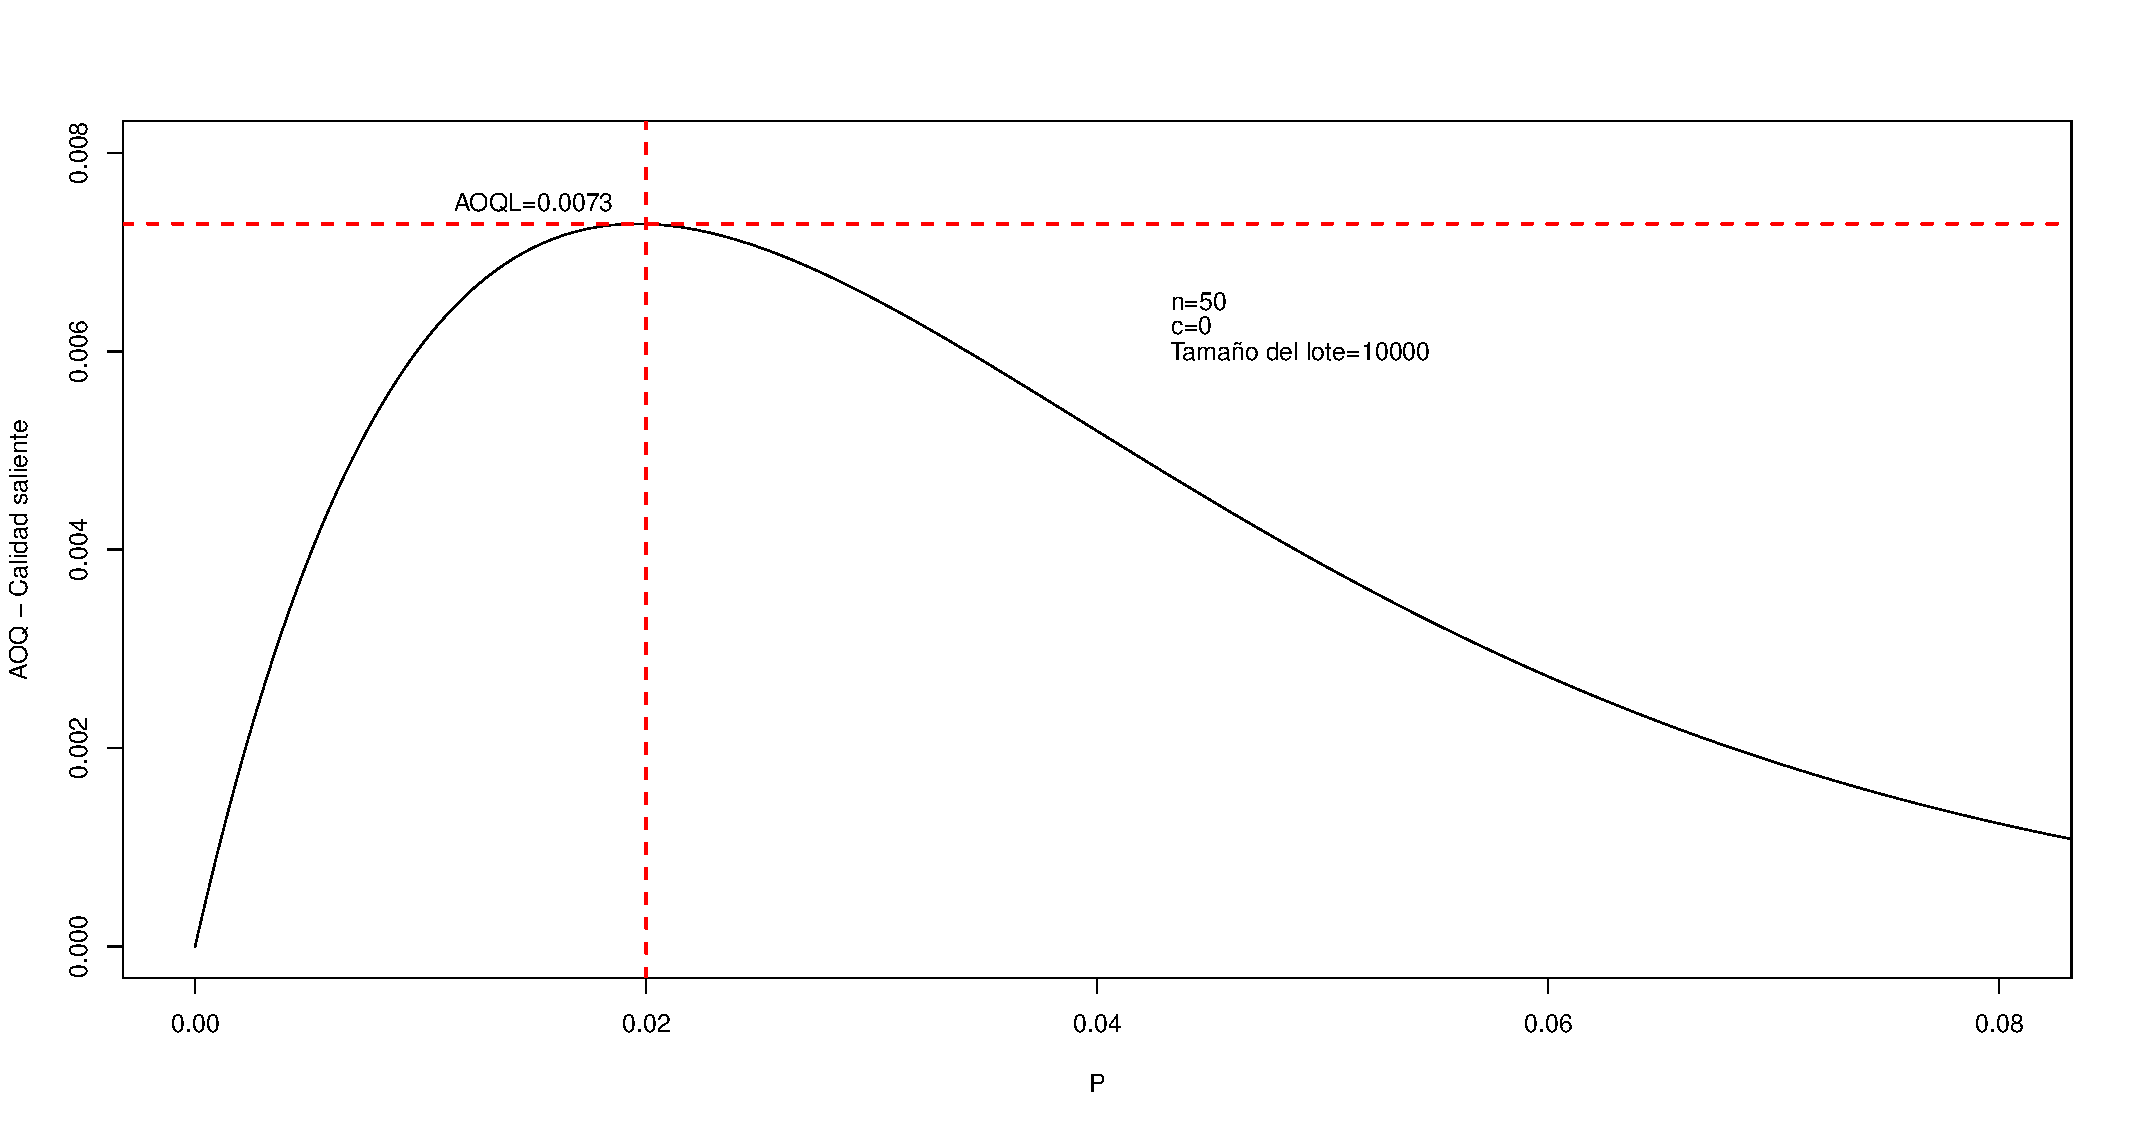
\includegraphics[scale=0.45]{IMAGENES/Figura2.pdf}
  \caption{Ejemplos curvas de operaci\'{o}n para lotes grandes $n/N<0.1$}
\end{figure}

~\\En el muestreo de aceptaci\'{o}n de lotes, se deben determinar ciertos par\'{a}metros que nos permitan decidir si rechazamos o aceptamos el lote a partir de los datos recogidos en la muestra, esos par\'{a}metros son:
\item N\'{u}mero de aceptaci\'{o}n: Es el n\'{u}mero de unidades infestadas o el n\'{u}mero de plagas individuales permitidas en una
muestra de determinado tama\~{n}o, antes de que se tomen medidas fitosanitarias.\cite{MUES}
\item Nivel de detecci\'{o}n:Es el porcentaje o la proporci\'{o}n de infestaci\'{o}n m\'{i}nimo que detectar\'{a} la metodolog\'{i}a de muestreo
al nivel de eficacia de detecci\'{o}n y el nivel de confianza especificado.\cite{MUES}
\item Nivel de confianza:Indica la probabilidad de que un env\'{i}o con un grado de infestaci\'{o}n que exceda el nivel de
detecci\'{o}n ser\'{a} detectado. Se suele utilizar un nivel de confianza del 95\%.\cite{MUES}
\item Eficacia de la detecci\'{o}n: La eficacia de la detecci\'{o}n es la probabilidad de que la inspecci\'{o}n o la prueba de diagn\'{o}stico de una o m\'{a}s unidades infestadas detectar\'{a} una plaga. En general, no deber\'{i}a suponerse que habr\'{a} un 100\% de eficacia.\cite{MUES}
\item Tama\~{n}o de la muestra: Es la cantidad de unidades seleccionadas del lote o env\'{i}o que se inspeccionar\'{a}n o someter\'{a}n a
pruebas de diagn\'{o}stico.\cite{MUES}
\item Nivel de tolerancia:Se refiere al porcentaje de infestaci\'{o}n de todo el env\'{i}o o lote que constituye el umbral para la acci\'{o}n fitosanitaria.En general, se utiliza un nivel de tolerancia 0.\cite{MUES}
\end{itemize}
